\section{Capítulo 4 -- Estruturas de decisão}

Até aqui, os programas executavam sempre os mesmos comandos, de cima para baixo, qualquer que fosse a entrada. Programas úteis precisam reagir aos dados: dar desconto só para compras acima de um valor, aprovar só quem atingiu a média, recusar uma senha errada. As \textbf{estruturas de decisão} (ou condicionais) escolhem quais comandos executar de acordo com uma condição. Neste capítulo você vai conhecer todas as formas de decisão do C++ e do Portugol, aprender a organizar decisões com várias alternativas e a evitar armadilhas que fazem o programa compilar, rodar e tomar a decisão errada.

\subsection{4.1 Decisão simples: if}

A \textbf{decisão simples} executa um bloco de comandos somente se uma condição for verdadeira; se for falsa, o bloco é pulado e o programa segue. A condição é qualquer expressão que resulte em verdadeiro ou falso, normalmente construída com os operadores relacionais e lógicos do Capítulo 3.

\begin{center}
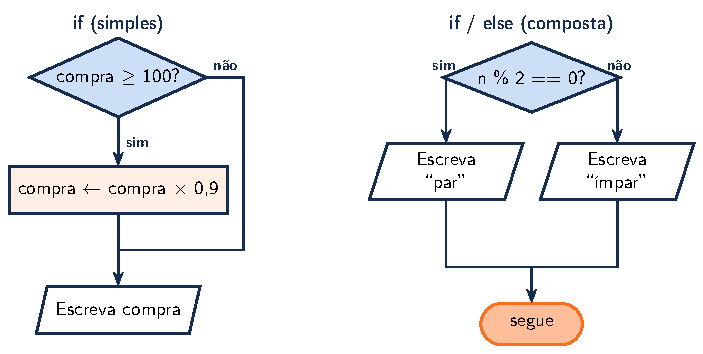
\includegraphics[width=0.85\linewidth,keepaspectratio]{imagens/capitulo-04_composta.pdf}
\end{center}

O fluxograma da esquerda corresponde a uma loja que dá 10\% de desconto em compras a partir de R\$ 100:

\begin{codigo}
\begin{Verbatim}[breaklines=true, breaksymbolleft={}, fontsize=\footnotesize]
algoritmo "Desconto"
var
   compra: real
inicio
   escreva("Valor da compra: ")
   leia(compra)
   se compra >= 100 entao
      compra <- compra * 0.9
      escreval("Você ganhou 10% de desconto!")
   fimse
   escreval("Total: R$ ", compra:8:2)
fimalgoritmo
\end{Verbatim}
\end{codigo}

\begin{codigo}
\begin{Verbatim}[breaklines=true, breaksymbolleft={}, fontsize=\footnotesize]
#include <iostream>
#include <iomanip>
using namespace std;

int main() {
    double compra;
    cout << "Valor da compra: ";
    cin >> compra;
    if (compra >= 100) {
        compra = compra * 0.9;         // 10% de desconto
        cout << "Você ganhou 10% de desconto!" << endl;
    }
    cout << fixed << setprecision(2) << "Total: R$ " << compra
         << endl;
    return 0;
}
\end{Verbatim}
\end{codigo}

Em C++, a condição fica \textbf{entre parênteses}, e os comandos controlados pelo \texttt{if} ficam entre chaves, formando um \textbf{bloco}. Se o bloco tiver um único comando, as chaves podem ser omitidas, mas é uma boa prática usá-las sempre: elas evitam que um comando acrescentado depois fique fora do \texttt{if} sem que ninguém perceba (Seção 4.7). No Portugol, o bloco termina com \texttt{fimse}.

\subsection{4.2 Decisão composta: if e else}

A \textbf{decisão composta} escolhe entre dois caminhos: um para quando a condição é verdadeira, outro para quando é falsa. Exatamente um deles é executado, nunca os dois e nunca nenhum. É o fluxograma da direita na figura anterior.

\begin{codigo}
\begin{Verbatim}[breaklines=true, breaksymbolleft={}, fontsize=\footnotesize]
#include <iostream>
using namespace std;

int main() {
    int n;
    cout << "Digite um número inteiro: ";
    cin >> n;
    if (n % 2 == 0) {
        cout << n << " é par" << endl;
    } else {
        cout << n << " é ímpar" << endl;
    }
    return 0;
}
\end{Verbatim}
\end{codigo}

Em Portugol, a parte do ``senão'' é escrita com \texttt{senao}, antes do \texttt{fimse}:

\begin{codigo}
\begin{Verbatim}[breaklines=true, breaksymbolleft={}, fontsize=\footnotesize]
algoritmo "ParOuImpar"
var
   n: inteiro
inicio
   escreva("Digite um número inteiro: ")
   leia(n)
   se n mod 2 = 0 entao
      escreval(n, " é par")
   senao
      escreval(n, " é ímpar")
   fimse
fimalgoritmo
\end{Verbatim}
\end{codigo}

\subsection{4.3 Decisões encadeadas: else if}

Muitos problemas têm mais de dois caminhos. A situação de um aluno, por exemplo, depende da média: inválida se estiver fora de 0 a 10, aprovado com 6 ou mais, prova final entre 4 e 6, reprovado abaixo de 4. Para isso, encadeiam-se várias decisões: cada \texttt{else} traz um novo \texttt{if}.

\begin{center}
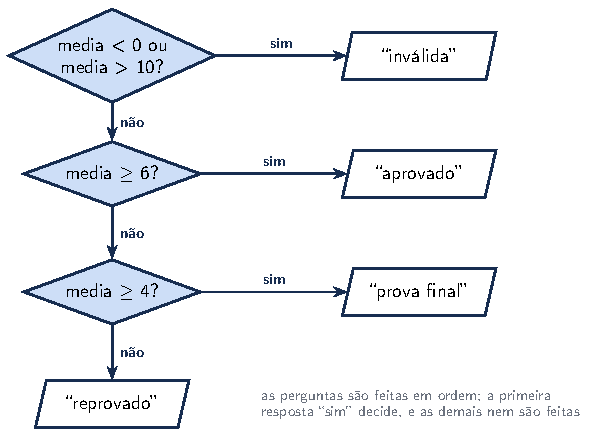
\includegraphics[width=0.75\linewidth,keepaspectratio]{imagens/capitulo-04_encadeada.pdf}
\end{center}

\begin{codigo}
\begin{Verbatim}[breaklines=true, breaksymbolleft={}, fontsize=\footnotesize]
#include <iostream>
using namespace std;

int main() {
    double media;
    cout << "Média final: ";
    cin >> media;
    if (media < 0 || media > 10) {
        cout << "Média inválida" << endl;
    } else if (media >= 6) {
        cout << "Aprovado" << endl;
    } else if (media >= 4) {
        cout << "Prova final" << endl;
    } else {
        cout << "Reprovado" << endl;
    }
    return 0;
}
\end{Verbatim}
\end{codigo}

As condições são testadas \textbf{em ordem}, e a primeira verdadeira decide: as seguintes nem são avaliadas. Por isso, a ordem importa. Quando o programa chega em \texttt{media >= 4}, já se sabe que a média não é maior ou igual a 6, senão o caminho anterior teria sido seguido; não é preciso escrever \texttt{media >= 4 \&\& media < 6}. Mas, se as duas condições fossem trocadas de lugar, uma média 9 cairia em ``prova final'', porque 9 também é maior ou igual a 4.

O Portugol do VisuAlg não tem uma palavra para ``senão se'': os \texttt{se} ficam um dentro do outro, cada um com o seu \texttt{fimse}.

\begin{codigo}
\begin{Verbatim}[breaklines=true, breaksymbolleft={}, fontsize=\footnotesize]
algoritmo "Situacao"
var
   media: real
inicio
   escreva("Média final: ")
   leia(media)
   se (media < 0) ou (media > 10) entao
      escreval("Média inválida")
   senao
      se media >= 6 entao
         escreval("Aprovado")
      senao
         se media >= 4 entao
            escreval("Prova final")
         senao
            escreval("Reprovado")
         fimse
      fimse
   fimse
fimalgoritmo
\end{Verbatim}
\end{codigo}

Para testar uma decisão encadeada, use pelo menos um valor de cada faixa e os valores exatamente nas fronteiras: $-1$, 0, 3.9, 4, 5.9, 6, 10 e 11. A fronteira é onde mora o erro de usar \texttt{>} no lugar de \texttt{>=}.

\subsection{4.4 Decisões aninhadas}

Uma decisão pode estar \textbf{dentro} de outra. Isso é útil quando uma pergunta só faz sentido depois que outra foi respondida. Para classificar um triângulo pelos lados, por exemplo, primeiro é preciso saber se os três lados formam um triângulo: cada lado tem de ser menor que a soma dos outros dois. Só então faz sentido perguntar se ele é equilátero, isósceles ou escaleno.

\begin{codigo}
\begin{Verbatim}[breaklines=true, breaksymbolleft={}, fontsize=\footnotesize]
#include <iostream>
using namespace std;

int main() {
    int a, b, c;
    cout << "Lados do triângulo: ";
    cin >> a >> b >> c;
    if (a < b + c && b < a + c && c < a + b) {
        if (a == b && b == c) {
            cout << "Equilátero" << endl;   // três iguais
        } else if (a == b || b == c || a == c) {
            cout << "Isósceles" << endl;    // dois iguais
        } else {
            cout << "Escaleno" << endl;     // todos diferentes
        }
    } else {
        cout << "Esses lados não formam um triângulo" << endl;
    }
    return 0;
}
// 3 3 3 -> Equilátero    5 5 8 -> Isósceles
// 3 4 5 -> Escaleno      1 2 10 -> não formam um triângulo
\end{Verbatim}
\end{codigo}

O recuo deixa visível o que está dentro de quê. Com muitos níveis de aninhamento, porém, o código fica difícil de ler. Muitas vezes é possível trocar decisões aninhadas por uma única condição composta: ``se tem nota e se tem frequência'' é o mesmo que ``se tem nota \textbf{e} frequência''.

\begin{codigo}
\begin{Verbatim}[breaklines=true, breaksymbolleft={}, fontsize=\footnotesize]
// trecho
if (media >= 6) {                      // aninhado
    if (frequencia >= 75) {
        cout << "Aprovado" << endl;
    }
}
if (media >= 6 && frequencia >= 75) {  // o mesmo, em um só if
    cout << "Aprovado" << endl;
}
\end{Verbatim}
\end{codigo}

\subsection{4.5 Escolha múltipla: switch}

Quando a decisão compara \textbf{uma única variável} com vários valores fixos, como a opção de um menu, o \texttt{switch} é mais claro que uma sequência de \texttt{else if}. Ele avalia a variável uma vez e salta direto para o \texttt{case} correspondente.

\begin{codigo}
\begin{Verbatim}[breaklines=true, breaksymbolleft={}, fontsize=\footnotesize]
#include <iostream>
using namespace std;

int main() {
    double a, b;
    char operacao;
    cout << "Conta (ex.: 8 * 3): ";
    cin >> a >> operacao >> b;
    switch (operacao) {
        case '+':
            cout << a + b << endl;
            break;
        case '-':
            cout << a - b << endl;
            break;
        case '*':
        case 'x':                  // dois casos, mesmo código
            cout << a * b << endl;
            break;
        case '/':
            if (b != 0) {
                cout << a / b << endl;
            } else {
                cout << "Divisão por zero" << endl;
            }
            break;
        default:                        // nenhum dos casos acima
            cout << "Operação desconhecida" << endl;
    }
    return 0;
}
// 8 * 3 -> 24        8 x 3 -> 24
// 7 / 2 -> 3.5       5 / 0 -> Divisão por zero
\end{Verbatim}
\end{codigo}

\begin{itemize}
  \item Cada \texttt{case} indica um valor possível. Ele precisa ser uma constante, de um tipo inteiro ou \texttt{char}: o \texttt{switch} não funciona com \texttt{double}, \texttt{string} nem com faixas como ``de 4 a 6''.
  \item O \texttt{break} encerra o \texttt{switch}. Sem ele, a execução \textbf{continua no caso seguinte}, mesmo que o valor seja outro. Às vezes isso é útil, como em \texttt{'*'} e \texttt{'x'}, que compartilham o mesmo código; na maioria das vezes, esquecer o \texttt{break} é um erro.
  \item O \texttt{default} é executado quando nenhum caso corresponde, e funciona como o \texttt{else} final.
\end{itemize}

No Portugol do VisuAlg, a mesma estrutura se chama \texttt{escolha}, e não precisa de \texttt{break}, porque cada caso termina sozinho:

\begin{codigo}
\begin{Verbatim}[breaklines=true, breaksymbolleft={}, fontsize=\footnotesize]
algoritmo "DiaDaSemana"
var
   dia: inteiro
inicio
   escreva("Dia (1 a 7): ")
   leia(dia)
   escolha dia
   caso 1, 7
      escreval("Fim de semana")
   caso 2, 3, 4, 5, 6
      escreval("Dia útil")
   outrocaso
      escreval("Dia inválido")
   fimescolha
fimalgoritmo
\end{Verbatim}
\end{codigo}

\subsection{4.6 O operador ternário}

Quando a decisão só escolhe entre \textbf{dois valores}, o \textbf{operador ternário} \texttt{?:} faz isso em uma linha: \texttt{condição ? valor\_se\_verdadeiro : valor\_se\_falso}. Ele não substitui o \texttt{if} em geral; serve para escolher um valor, e não para executar blocos de comandos.

O programa completo deste capítulo usa o ternário para verificar se um ano é \textbf{bissexto}. Pelo calendário gregoriano, um ano é bissexto se for divisível por 4, exceto os divisíveis por 100, que só são bissextos se também forem divisíveis por 400. Por isso 2024 e 2000 foram bissextos, mas 1900 não foi.

\begin{codigo}
\begin{Verbatim}[breaklines=true, breaksymbolleft={}, fontsize=\footnotesize]
#include <iostream>
using namespace std;

int main() {
    int ano;
    cout << "Ano: ";
    cin >> ano;
    bool bissexto = (ano % 4 == 0 && ano % 100 != 0)
                    || ano % 400 == 0;
    int dias = bissexto ? 366 : 365;
    cout << ano << (bissexto ? " é" : " não é")
         << " bissexto e tem " << dias << " dias" << endl;
    return 0;
}
// 2024 é bissexto e tem 366 dias
// 1900 não é bissexto e tem 365 dias
\end{Verbatim}
\end{codigo}

Repare que a regra inteira cabe em uma única expressão lógica, guardada na variável \texttt{bissexto}. Dar um nome à condição deixa o resto do programa muito mais legível do que repetir a expressão em cada \texttt{if}. Um teste de mesa com os casos que exercitam cada parte da regra:

\begin{center}
\begin{tabular}{@{}p{0.13\linewidth}p{0.13\linewidth}p{0.15\linewidth}p{0.15\linewidth}p{0.27\linewidth}@{}}
\toprule
\rowcolor{headergray}
\tblheader{Ano} & \tblheader{\% 4} & \tblheader{\% 100} & \tblheader{\% 400} & \tblheader{Bissexto?} \\
\midrule
2023 & 3 & 23 & 23 & não (não divide por 4) \\
\rowcolor{rowgray} 2024 & 0 & 24 & 24 & sim \\
1900 & 0 & 0 & 300 & não (divide por 100) \\
\rowcolor{rowgray} 2000 & 0 & 0 & 0 & sim (divide por 400) \\
\bottomrule
\end{tabular}
\end{center}

\subsection{4.7 Armadilhas das decisões}

Alguns erros com decisões passam pela compilação e só aparecem no resultado. O programa abaixo tem dois deles:

\begin{codigo}
\begin{Verbatim}[breaklines=true, breaksymbolleft={}, fontsize=\footnotesize]
// erro: dois enganos que o compilador aceita
int main() {
    int saldo = 50;
    if (saldo = 0) {                  // = no lugar de ==
        cout << "Sem saldo" << endl;
    }
    if (saldo > 100);                 // ; logo depois do if
    {
        cout << "Saldo alto" << endl;
    }
    cout << saldo << endl;
    return 0;
}
// Saída: Saldo alto
//        0
\end{Verbatim}
\end{codigo}

\begin{itemize}
  \item Em \texttt{if (saldo = 0)}, o \texttt{=} \textbf{atribui} 0 ao saldo, em vez de compará-lo. O valor da atribuição, 0, é tratado como falso, então ``Sem saldo'' não aparece, mas o saldo foi zerado.
  \item Em \texttt{if (saldo > 100);}, o ponto e vírgula encerra o \texttt{if} com um comando vazio. O bloco entre chaves logo abaixo deixa de pertencer a ele e é executado sempre. Resultado: ``Saldo alto'' com saldo 0.
\end{itemize}

Os dois erros são avisados pelo g++ quando se compila com \texttt{-Wall -Wextra}: ``\texttt{suggest parentheses around assignment used as truth value}'' para o primeiro e ``\texttt{suggest braces around empty body in an 'if' statement}'' para o segundo. É mais um motivo para nunca ignorar os avisos.

Um terceiro cuidado é o \texttt{else} sem chaves. Sem elas, cada \texttt{if} controla apenas o comando seguinte, e um \texttt{else} sempre pertence ao \texttt{if} mais próximo que ainda não tem \texttt{else}, não importa o recuo. Com chaves em todos os blocos, essa dúvida simplesmente não existe.

\subsection{Erros Comuns}

\begin{itemize}
  \item \textbf{Usar \texttt{=} na condição.} \texttt{if (x = 5)} atribui e é quase sempre verdadeiro. Para comparar, use \texttt{==}.
  \item \textbf{Colocar ponto e vírgula depois do \texttt{if}.} \texttt{if (cond);} encerra a decisão ali, e o bloco seguinte é executado sempre.
  \item \textbf{Omitir as chaves.} Um segundo comando acrescentado depois fica fora do \texttt{if}, mesmo com o recuo certo. Use chaves sempre.
  \item \textbf{Ordenar mal as condições encadeadas.} Testar \texttt{media >= 4} antes de \texttt{media >= 6} faz toda média alta cair no caso errado. Do mais restritivo para o menos restritivo.
  \item \textbf{Esquecer o \texttt{break} no \texttt{switch}.} A execução continua nos casos seguintes.
  \item \textbf{Usar \texttt{switch} com faixas ou textos.} Cada \texttt{case} é um valor exato, inteiro ou \texttt{char}. Para faixas, use \texttt{else if}.
  \item \textbf{Esquecer um caso.} Pergunte sempre o que acontece com os valores fora do esperado: média negativa, divisão por zero, opção inexistente do menu. Use \texttt{else} e \texttt{default} para tratá-los.
  \item \textbf{Testar só um caminho.} Cada ramo da decisão precisa de pelo menos um teste, e cada fronteira, de um valor exatamente nela.
\end{itemize}
